\chapter{Thermodynamics of Electrochemical Cells}\label{ch:b2:cell-thermodynamics}

A hydrogen fuel-cell bus carries a stack of a few hundred thin cells. In each,
hydrogen and the oxygen of the air combine to water without a flame, and the
energy comes out as an electric current. Two numbers govern such a stack, and
both come straight from tables of Gibbs energies: no cell can give more than
\qty{1.23}{V}, and no fuel cell, however perfect, turns all the energy of its
hydrogen into electrical work. This chapter connects the voltage of a cell to
the \omterm{def:b2:reaction-free-energy:gibbs-energy}{Gibbs energy} of its reaction, derives the Nernst equation used since the
Year 1 volume, and reads entropies and enthalpies of reaction off a voltmeter
and a thermometer.

\begin{recall}
The Year 1 volume: cells, half-cells, anode and cathode, salt bridge, cell
voltage, electrode potential, standard potential and the standard hydrogen
electrode, the Nernst equation (admitted there), equilibrium constants from
potentials. \Cref{ch:b2:reaction-free-energy}: $\Delta_r G$, $\Delta_r G^\circ$
and $\Delta_r G = \Delta_r G^\circ + RT\ln Q$; the evolution criterion.
\Cref{ch:b2:chemical-potential}: activities. The school volume: electrolysis.
\end{recall}

\begin{omfigure}
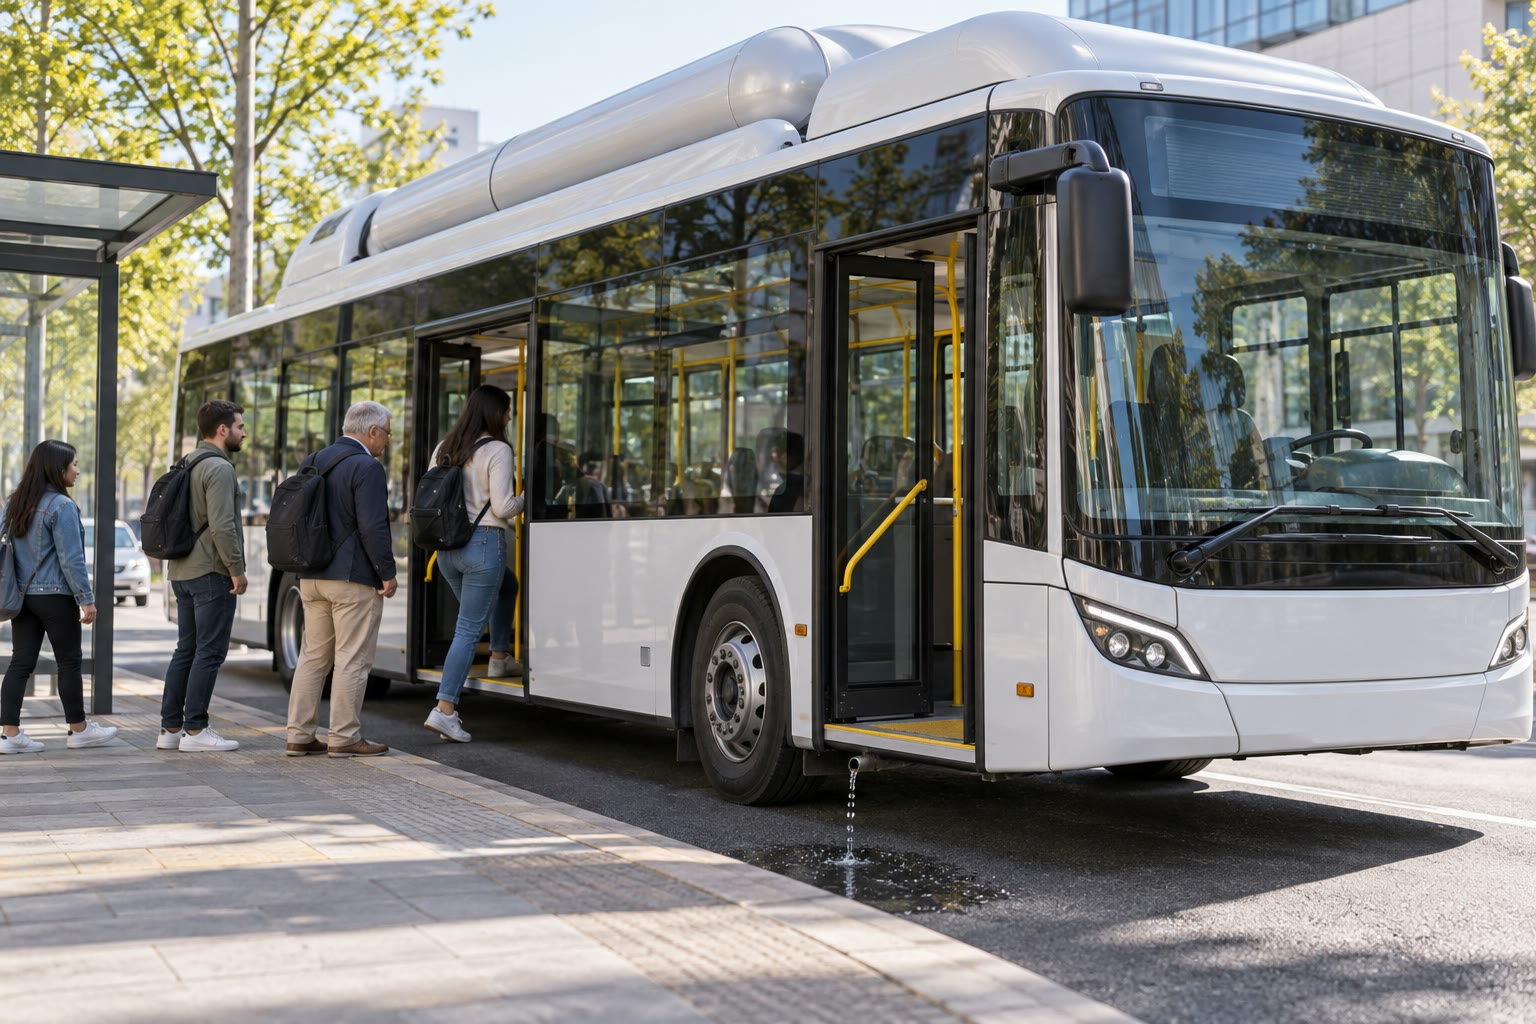
\includegraphics[width=0.62\linewidth]{images/book3/ai/b2-09-fuel-cell-bus.jpg}

{\small A hydrogen fuel-cell bus at a stop: the hydrogen tanks are under the
fairing on the roof, and the only exhaust is water, dripping under the bus.}
\end{omfigure}

\section{Electrical work and the Faraday constant}

\begin{definition}[Faraday constant]\label{def:b2:cell-thermodynamics:faraday}
The \emph{Faraday constant}\index{Faraday constant} is the electric charge of
one mole of elementary charges, $F = N_A e = \qty{96485.33}{C/mol}$.
% ledger: const:F
\end{definition}

\begin{proposition}[Charge passed]\label{prop:b2:cell-thermodynamics:charge}
If the reaction of a cell, written with $n$ electrons exchanged, advances by
$\Delta\xi$, the charge that flows through the external circuit is $Q =
nF\,\Delta\xi$.
\end{proposition}

\begin{proof}
An advancement $\Delta\xi$ transfers $n\,\Delta\xi$ moles of electrons from
the anode to the cathode through the wire, each of charge $e$ in magnitude:
$Q = n\,\Delta\xi\,N_A e$.
\end{proof}

When a charge $Q$ is driven through a circuit by a voltage $U$, the work
received by the circuit is $QU$. Seen from the cell, which delivers that work,
the electrical work it receives is $\delta W_{\text{el}} = -U\,\delta Q = -nFU\,
d\xi$.

\begin{omfigure}
\begin{tikzpicture}[font=\small, >={Stealth}]
  \draw[thick, rounded corners, fill=omDef!8] (0,0) rectangle (3.2,2.2);
  \node[align=center] at (1.6,1.1) {cell\\ (system)\\ reaction $d\xi$};
  \draw[->, thick, omThm] (3.2,1.6) -- (5.6,1.6) node[right, align=left] {$\delta W_{\text{el}}$ delivered\\ $= nFU\,d\xi$};
  \draw[->, thick, omDef] (5.6,0.6) -- (3.2,0.6) node[pos=0, right, align=left] {$\delta Q_{\text{heat}}$ received\\ (sign either way)};
  \draw[<->, thick] (1.6,2.2) -- (1.6,3.0) node[above] {surroundings at $T$, $p$};
\end{tikzpicture}

{\small A cell as a thermodynamic system at constant temperature and pressure:
it exchanges heat with its surroundings and delivers electrical work through
the external circuit. With the sign convention of the first law (work and heat
received counted positive), $\delta W_{\text{el}} = -nFU\,d\xi$.}
\end{omfigure}

\section{The Gibbs energy of a cell reaction}

\begin{theorem}[Electrical work and Gibbs energy]\label{thm:b2:cell-thermodynamics:delta-g-nfe}
A cell working at constant $T$ and $p$ delivers an electrical work at most
equal to the decrease of its \omterm{def:b2:reaction-free-energy:gibbs-energy}{Gibbs energy}: for an advancement $d\xi$,
$nFU\,d\xi \leq -\Delta_r G\,d\xi$. When it works reversibly (an
infinitesimal current), the equality holds, and the cell voltage is the
electromotive force
\[
  \Delta_r G = -nFE .
\]
\end{theorem}

\begin{proof}
First law at constant pressure, with the pressure work separated:
$dH = \delta Q + \delta W_{\text{el}}$. Second law: $dS \geq \delta Q/T$. At
constant $T$ and $p$, $dG = dH - T\,dS \leq \delta W_{\text{el}} = -nFU\,d\xi$.
With $dG = \Delta_r G\,d\xi$, $\Delta_r G\,d\xi \leq -nFU\,d\xi$, that is
$nFU\,d\xi \leq -\Delta_r G\,d\xi$. For a reversible change the inequality
of the second law is an equality, and the voltage then measured, with no
current, is $E$: $\Delta_r G = -nFE$.
\end{proof}

A cell can thus run forward ($d\xi > 0$, delivering work) only if $\Delta_r G <
0$, that is $E > 0$ with the poles chosen so that the reaction written runs
from anode to cathode. A real cell, through which a current flows, delivers
less work than $-\Delta_r G$: the difference is dissipated as heat in its
resistance and at its electrodes (\cref{ch:b2:current-potential-curves}).

\begin{example}[The Daniell cell]\label{ex:b2:cell-thermodynamics:daniell}
For \ce{Zn + Cu^2+ -> Zn^2+ + Cu}, $\Delta_r G^\circ = \Delta_f G^\circ(\ce{Zn^2+}) -
\Delta_f G^\circ(\ce{Cu^2+}) = -147.06 - 65.49 = \qty{-212.55}{kJ/mol}$, and $n = 2$:
$E^\circ = 212\,550/(2 \times 96\,485) = \qty{1.10}{V}$, the voltage measured on a
Daniell cell in standard conditions.
% ledger: dfg:Zn2+_ao, dfg:Cu2+_ao, const:F, emf:Daniell
\end{example}

\section{The Nernst equation and standard potentials}

The Year 1 volume admitted the Nernst equation; it now follows from
$\Delta_r G = \Delta_r G^\circ + RT\ln Q$.

\begin{theorem}[The Nernst equation, derived]\label{thm:b2:cell-thermodynamics:nernst-derived}
For a half-reaction $\alpha\,\mathrm{Ox} + n\,\mathrm e^- \rightleftharpoons
\beta\,\mathrm{Red}$, the potential of the electrode at temperature $T$ is
\[
  E = E^\circ + \frac{RT}{nF}\ln\frac{a_{\mathrm{Ox}}^{\alpha}}{a_{\mathrm{Red}}^{\beta}} ,
\]
where the activities include those of every other species of the
half-reaction (\ce{H+}, water excepted), with their stoichiometric powers.
\end{theorem}

\begin{proof}
The potential of an electrode is the voltage of the cell made of the standard
hydrogen electrode (anode) and that electrode (cathode). Its reaction is
\[
  \alpha\,\mathrm{Ox} + \tfrac n2\,\ce{H2} \longrightarrow \beta\,\mathrm{Red} + n\,\ce{H+} ,
\]
whose reaction quotient, with $a_{\ce{H+}} = 1$ and $p_{\ce{H2}} = p^\circ$ at
the standard hydrogen electrode, reduces to $a_{\mathrm{Red}}^\beta/
a_{\mathrm{Ox}}^\alpha$. From \cref{thm:b2:cell-thermodynamics:delta-g-nfe},
$E = -\Delta_r G/(nF) = -\Delta_r G^\circ/(nF) - (RT/nF)\ln Q$; with $E^\circ =
-\Delta_r G^\circ/(nF)$ this is the formula. At \qty{298.15}{K}, $RT\ln 10/F =
\qty{0.0592}{V}$.
\end{proof}

\begin{proposition}[Standard potentials from Gibbs energies]\label{prop:b2:cell-thermodynamics:standard-potential}
With the conventions $\Delta_f G^\circ(\ce{H+}, \text{aq}) = 0$ and
$\Delta_f G^\circ(\ce{H2}, \text{g}) = 0$, the standard potential of a couple is
$E^\circ = -\Delta_r G^\circ/(nF)$, where $\Delta_r G^\circ$ is the standard \omterm{def:b2:reaction-free-energy:gibbs-energy}{Gibbs
energy} of the half-reaction written as a reduction, the electrons counted as
having zero \omterm{def:b2:reaction-free-energy:gibbs-energy}{Gibbs energy}.
\end{proposition}

\begin{proof}
In the reaction against the hydrogen electrode, $\tfrac n2\,\ce{H2}$ and
$n\,\ce{H+}$ contribute nothing to $\Delta_r G^\circ$ under those conventions: the
standard \omterm{def:b2:reaction-free-energy:gibbs-energy}{Gibbs energy} of the cell reaction is that of the half-reaction alone.
\end{proof}

\begin{method}[A standard potential from tables]\label{met:b2:cell-thermodynamics:e-from-gibbs}
\begin{enumerate}
  \item Write the half-reaction as a reduction, balanced with \ce{H+} and
        \ce{H2O}, with $n$ electrons.
  \item Compute $\Delta_r G^\circ = \sum\nu_i\Delta_f G^\circ_i$ (products
        positive), with zero for the elements, \ce{H+} and the electrons.
  \item $E^\circ = -\Delta_r G^\circ/(nF)$, in volts with $\Delta_r G^\circ$ in
        joules per mole.
\end{enumerate}
\end{method}

\begin{example}[The silver chloride electrode]\label{ex:b2:cell-thermodynamics:agcl}
\ce{AgCl(s) + e- -> Ag(s) + Cl^-}: $\Delta_r G^\circ = -131.228 - (-109.789) =
\qty{-21.439}{kJ/mol}$, $E^\circ = 21\,439/96\,485 = \qty{0.222}{V}$. Its potential
depends on the chloride activity only: in a saturated potassium chloride
solution it is a stable reference electrode.
% ledger: dfg:Cl-_ao, dfg:AgCl_cr
\end{example}

\begin{proposition}[Combining potentials]\label{prop:b2:cell-thermodynamics:combining}
If a half-reaction (3), with $n_3$ electrons, is the sum of half-reactions (1)
and (2), with $n_1$ and $n_2$ electrons, then
\[
  n_3E_3^\circ = n_1E_1^\circ + n_2E_2^\circ ;
\]
the potentials themselves do not add.
\end{proposition}

\begin{proof}
Standard Gibbs energies add, $\Delta_r G_3^\circ = \Delta_r G_1^\circ + \Delta_r
G_2^\circ$, and the electron counts add, $n_3 = n_1 + n_2$. Divide each $\Delta_r
G^\circ$ by $-F$.
\end{proof}

\begin{example}[Iron in its two oxidation states]\label{ex:b2:cell-thermodynamics:iron}
\ce{Fe^3+ + e- -> Fe^2+} has $E^\circ = (-78.90 + 4.7)/(-96.485) = \qty{0.77}{V}$
and \ce{Fe^2+ + 2e- -> Fe} has $E^\circ = -78.90/(2 \times 96.485) =
\qty{-0.41}{V}$. Hence \ce{Fe^3+ + 3e- -> Fe}: $E^\circ = (0.77 - 0.82)/3 =
\qty{-0.02}{V}$, not the sum of the two.
% ledger: dfg:Fe2+_ao, dfg:Fe3+_ao
\end{example}

\section{Temperature, entropy and the efficiency of a fuel cell}

\begin{definition}[Temperature coefficient]\label{def:b2:cell-thermodynamics:temperature-coefficient}
The \emph{temperature coefficient}\index{temperature coefficient} of a cell is
the derivative $(\partial E/\partial T)_p$ of its electromotive force with
respect to temperature.
\end{definition}

\begin{proposition}[Entropy and enthalpy from cell data]\label{prop:b2:cell-thermodynamics:entropy}
For the standard cell reaction,
\[
  \Delta_r S^\circ = nF\,\frac{dE^\circ}{dT}, \qquad
  \Delta_r H^\circ = -nF\Big(E^\circ - T\frac{dE^\circ}{dT}\Big),
\]
and a cell working reversibly at temperature $T$ receives from its
surroundings the heat $T\Delta_r S$ per mole of reaction.
\end{proposition}

\begin{proof}
$\Delta_r S^\circ = -d\Delta_r G^\circ/dT$ (from $dG = -S\,dT + V\,dp$, differentiated
with respect to $\xi$) $= nF\,dE^\circ/dT$; then $\Delta_r H^\circ = \Delta_r G^\circ
+ T\Delta_r S^\circ$. For the reversible change, $\delta Q = T\,dS = T\Delta_r S\,
d\xi$.
\end{proof}

\begin{method}[From cell data to the thermodynamics of the reaction]\label{met:b2:cell-thermodynamics:cell-data}
\begin{enumerate}
  \item Measure $E$ at several temperatures; the slope is $dE/dT$.
  \item $\Delta_r G = -nFE$, $\Delta_r S = nF\,dE/dT$, $\Delta_r H = \Delta_r G +
        T\Delta_r S$.
  \item Heat exchanged per mole when the cell works reversibly: $T\Delta_r S$;
        when it delivers a current at a voltage $U < E$, the heat released is
        $-\Delta_r H - nFU$ per mole.
\end{enumerate}
\end{method}

For the hydrogen--oxygen cell producing liquid water, the CODATA key values
give $\Delta_r H^\circ = \qty{-285.83}{kJ/mol}$ and
\[
  \Delta_r S^\circ = 69.95 - 130.68 - \tfrac12 \times 205.15 = \qty{-163.3}{J/(K.mol)} ,
\]
so $\Delta_r G^\circ = \qty{-237.14}{kJ/mol}$ and $E^\circ = \qty{1.229}{V}$; the
\omterm{def:b2:cell-thermodynamics:temperature-coefficient}{temperature coefficient} is $\Delta_r S^\circ/(2F) = \qty{-0.85}{mV/K}$. A hydrogen fuel cell gives less
voltage hot than cold.
% ledger: dfh:H2O-l, s0:H2O_l, s0:H2_g, s0:O2_g, janafG:H2O_l.298

\begin{omfigure}
\begin{tikzpicture}
\begin{axis}[width=0.48\linewidth, height=5.4cm, xmin=280, xmax=1020,
  ymin=0.95, ymax=1.26, axis x line=bottom, axis y line=left,
  xlabel={$T$ (K)}, ylabel={$E^\circ$ (V)}, tick label style={font=\small},
  label style={font=\small}, title={\small standard voltage}]
\addplot[omDef, thick, mark=*, mark size=1.2pt] table[x=T, y=E] {figdata/out/bachelor-2-cell-thermodynamics-a-liquid.dat};
\addplot[omThm, thick, mark=*, mark size=1.2pt] table[x=T, y=E] {figdata/out/bachelor-2-cell-thermodynamics-a-gas.dat};
\node[font=\scriptsize, omDef, anchor=north east] at (axis cs:480,1.05) {liquid water};
\node[font=\scriptsize, omThm, anchor=south west] at (axis cs:560,1.12) {water vapour};
\end{axis}
\end{tikzpicture}\hfill
\begin{tikzpicture}
\begin{axis}[width=0.48\linewidth, height=5.4cm, xmin=280, xmax=1520,
  ymin=0, ymax=1.0, axis x line=bottom, axis y line=left,
  xlabel={$T$ (K)}, ylabel={efficiency}, tick label style={font=\small},
  label style={font=\small}, title={\small maximum efficiency}]
\addplot[omThm, thick, mark=*, mark size=1.2pt] table[x=T, y=eta] {figdata/out/bachelor-2-cell-thermodynamics-b.dat};
\addplot[black!60, thick, dashed] table[x=T, y=eta] {figdata/out/bachelor-2-cell-thermodynamics-b-carnot.dat};
\node[font=\scriptsize, omThm, anchor=south] at (axis cs:700,0.87) {fuel cell};
\node[font=\scriptsize, black!70, anchor=north west] at (axis cs:520,0.40) {Carnot, $T_0 = \qty{298}{K}$};
\end{axis}
\end{tikzpicture}

{\small The hydrogen--oxygen cell from the JANAF tables. Left: standard voltage
$-\Delta_r G^\circ/(2F)$ with liquid water (up to \qty{500}{K}, the liquid kept
under its standard state) and with water vapour. Right: maximum efficiency
$\Delta_r G^\circ/\Delta_r H^\circ$ of the cell producing vapour, against the Carnot
efficiency of a heat engine working between $T$ and \qty{298}{K}; the engine
wins only above about \qty{1150}{K}.}
% ledger: janafG:H2O_l.298, janafG:H2O_l.300, janafG:H2O_l.400, janafG:H2O_l.500, janafG:H2O.298, janafG:H2O.300, janafG:H2O.400, janafG:H2O.500, janafG:H2O.600, janafG:H2O.700, janafG:H2O.800, janafG:H2O.900, janafG:H2O.1000, janafdfH:H2O_g.300, janafdfH:H2O_g.400, janafdfH:H2O_g.500, janafdfH:H2O_g.600, janafdfH:H2O_g.700, janafdfH:H2O_g.800, janafdfH:H2O_g.900, janafdfH:H2O_g.1000, janafdfH:H2O_g.1100, janafdfH:H2O_g.1300, janafdfH:H2O_g.1500, janafG:H2O.1100, janafG:H2O.1300, janafG:H2O.1500
\end{omfigure}

\begin{definition}[Thermodynamic efficiency of a fuel cell]\label{def:b2:cell-thermodynamics:efficiency}
The \emph{thermodynamic efficiency}\index{thermodynamic efficiency} of a fuel
cell is the ratio of the electrical work it delivers to the heat its fuel
would release by combustion at the same temperature, $-\Delta_r H$ per mole.
\end{definition}

\begin{proposition}[Maximum efficiency of a fuel cell]\label{prop:b2:cell-thermodynamics:efficiency}
The \omterm{def:b2:cell-thermodynamics:efficiency}{thermodynamic efficiency} of a fuel cell is at most $\Delta_r G/\Delta_r H$,
reached when it works reversibly, and equal to $(nFU)/(-\Delta_r H)$ at a working
voltage $U$. Unlike a heat engine, it is not limited by the Carnot efficiency
$1 - T_0/T$.
\end{proposition}

\begin{proof}
By \cref{thm:b2:cell-thermodynamics:delta-g-nfe} the work per mole is $nFU \leq
-\Delta_r G$; divide by $-\Delta_r H$. The cell converts chemical energy directly
into work at a single temperature: no heat is taken from a hot source and
partly given to a cold one, so the Carnot bound, which concerns such cycles,
does not apply. Its own bound is set by $T\Delta_r S$, the heat the reversible
cell must exchange.
\end{proof}

\begin{omfigure}
\begin{tikzpicture}[font=\small, x=0.022cm, y=0.6cm]
  \draw[->] (0,0) -- (320,0) node[right, font=\scriptsize] {\unit{kJ/mol}};
  \foreach \v in {0,100,200,300} \draw (\v,0) -- (\v,-0.12) node[below, font=\scriptsize] {\v};
  \fill[omThm!70] (0,2.2) rectangle (285.83,2.8);
  \node[anchor=west, font=\scriptsize] at (290,2.5) {$-\Delta_r H^\circ = 285.8$: heat of combustion};
  \fill[omDef!70] (0,1.2) rectangle (237.14,1.8);
  \fill[omProp!70] (237.14,1.2) rectangle (285.83,1.8);
  \node[anchor=west, font=\scriptsize] at (290,1.5) {$-\Delta_r G^\circ = 237.1$ work $+$ $48.7$ heat};
  \fill[omDef!40] (0,0.2) rectangle (135.1,0.8);
  \fill[omProp!40] (135.1,0.2) rectangle (285.83,0.8);
  \node[anchor=west, font=\scriptsize] at (290,0.5) {at \qty{0.70}{V}: $135.1$ work $+$ $150.7$ heat};
\end{tikzpicture}

{\small Where the energy of one mole of hydrogen goes in a fuel cell at
\qty{298}{K} (liquid water). Top: the heat a flame would release. Middle: the
reversible cell, which must give up $-T\Delta_r S^\circ = \qty{48.7}{kJ}$ as heat
whatever its design. Bottom: a real cell working at \qty{0.70}{V}.}
% ledger: dfh:H2O-l, s0:H2O_l, s0:H2_g, s0:O2_g, const:F
\end{omfigure}

\begin{history}[Faraday's laws of electrolysis]
\begin{minipage}[t]{0.27\linewidth}
\vspace{0pt}

\includegraphics[width=\linewidth]{images/book3/faraday.jpg}
\end{minipage}\hfill
\begin{minipage}[t]{0.69\linewidth}
\vspace{0pt}
In 1834 Michael Faraday, measuring the products of electrolyses with a
voltameter of his own design, stated that the mass of a substance produced
at an electrode is proportional to the quantity of electricity passed, and
that for a given quantity of electricity the masses of different substances
are in the ratio of their chemical equivalents. He coined the words
electrode, anode, cathode, ion, anion and cation. The constant that bears his
name turns those laws into $Q = nF\,\Delta\xi$. (Portrait by Thomas Phillips,
1842, public domain, Wikimedia Commons.)
\end{minipage}
\end{history}

\section{Concentration cells}

\begin{definition}[Concentration cell]\label{def:b2:cell-thermodynamics:concentration-cell}
A \emph{concentration cell}\index{concentration cell} is made of two
half-cells of the same couple that differ only in the concentration (or
pressure) of one species.
\end{definition}

\begin{proposition}[Voltage of a concentration cell]\label{prop:b2:cell-thermodynamics:concentration-cell}
Two electrodes of a metal M dipping into solutions of \ce{M^{n+}} at
concentrations $c_1 < c_2$, joined by a salt bridge, give a voltage
\[
  U = \frac{RT}{nF}\ln\frac{c_2}{c_1} ,
\]
the positive pole being the more concentrated side. The cell works until the
two concentrations are equal.
\end{proposition}

\begin{proof}
By the Nernst equation each electrode has $E_i = E^\circ + (RT/nF)\ln c_i$ (\omterm{def:b2:chemical-potential:ideal-mixture}{ideal
dilute solutions}); $E^\circ$ cancels in the difference. The reaction is
\ce{M^{n+}}(side 2) $\to$ \ce{M^{n+}}(side 1): metal is deposited on the
concentrated side (cathode) and dissolved on the dilute side (anode), which
evens the concentrations out; $\Delta_r G = RT\ln(c_1/c_2) < 0$ until they are
equal.
\end{proof}

\begin{omfigure}
\begin{tikzpicture}[font=\small, >={Stealth}]
  \pic at (0,0) {beaker={0.7}{omDef!10}};
  \pic at (3.6,0) {beaker={0.7}{omDef!32}};
  \pic at (-0.3,0.25) {electrode={black!25}};
  \pic at (3.9,0.25) {electrode={black!25}};
  \pic at (0.35,0.55) {saltbridge={2.9}};
  \pic (m) at (1.8,4.3) {meter={V}};
  % common (black) terminal on the anode side, red (+) on the cathode side
  \fill[black] (1.4,4.03) circle (0.065); \fill[red!70!black] (2.2,4.03) circle (0.065);
  \draw[thick] (-0.15,2.65) |- (m-a);
  \draw[thick] (4.05,2.65) |- (m-b);
  \node[anchor=east] at (-0.95,1.0) {\ce{Ag}};
  \node[anchor=west] at (4.45,1.0) {\ce{Ag}};
  \node at (0.25,-0.35) {\ce{Ag+} \qty{0.010}{mol/L}};
  \node at (3.6,-0.35) {\ce{Ag+} \qty{0.10}{mol/L}};
  \node[anchor=east] at (-0.9,2.3) {$-$ anode};
  \node[anchor=west] at (4.6,2.3) {cathode $+$};
  \node[font=\scriptsize] at (-0.1,-0.8) {\ce{Ag -> Ag+ + e-}};
  \node[font=\scriptsize] at (3.7,-0.8) {\ce{Ag+ + e- -> Ag}};
  \node[font=\scriptsize] at (1.8,5.05) {$U = \qty{59}{mV}$};
\end{tikzpicture}

{\small A silver \omterm{def:b2:cell-thermodynamics:concentration-cell}{concentration cell} at \qty{25}{\degreeCelsius}. The dilute side is
the anode: silver dissolves there and is deposited on the concentrated side,
until the two concentrations are equal. $U = 0.0592\log(0.10/0.010) =
\qty{59}{mV}$.}
\end{omfigure}

The same principle measures concentrations. A glass electrode, whose thin
membrane separates a reference solution from the sample, develops a membrane
potential of $(RT/F)\ln 10 = \qty{59}{mV}$ per unit of pH difference at
\qty{25}{\degreeCelsius}: the pH meter of the Year 1 volume is a \omterm{def:b2:cell-thermodynamics:concentration-cell}{concentration cell}
for \ce{H+}. Across the membrane of a living cell, the unequal concentrations
of \ce{K+} create in the same way a potential of several tens of millivolts.

\section{Exercises}

\begin{exercise}[$\star$]\label{exo:b2:cell-thermodynamics:1}
From $\Delta_f G^\circ(\ce{H2O}, \text{l}) = \qty{-237.14}{kJ/mol}$, compute the
standard voltage of the hydrogen--oxygen cell.
\end{exercise}

\begin{exercise}[$\star$]\label{exo:b2:cell-thermodynamics:2}
A battery is rated \qty{1.0}{A.h}. Compute the charge it holds, in coulombs,
and the mass of zinc consumed at its anode (\ce{Zn -> Zn^2+ + 2e-}) when it is
fully discharged.
\end{exercise}

\begin{exercise}[$\star$]\label{exo:b2:cell-thermodynamics:3}
A Daniell cell delivers \qty{1.10}{V} with no current. Compute $\Delta_r G$ for one
mole of zinc and the maximum electrical work for \qty{10.0}{g} of zinc.
\end{exercise}

\begin{exercise}[$\star$]\label{exo:b2:cell-thermodynamics:4}
Two copper electrodes dip into copper(II) sulfate solutions of \qty{1.0e-3}{mol/L}
and \qty{0.10}{mol/L}. Compute the voltage at \qty{25}{\degreeCelsius} and name the
poles.
\end{exercise}

\begin{exercise}[$\star\star$]\label{exo:b2:cell-thermodynamics:5}
A cell ($n = 2$) has $E^\circ = \qty{1.015}{V}$ and $dE^\circ/dT = \qty{-4.0e-4}{V/K}$
at \qty{298}{K} (exercise data). Compute $\Delta_r G^\circ$, $\Delta_r S^\circ$ and
$\Delta_r H^\circ$.
\end{exercise}

\begin{exercise}[$\star\star$]\label{exo:b2:cell-thermodynamics:6}
The cell of \cref{exo:b2:cell-thermodynamics:5} discharges one mole of reaction
(a) reversibly; (b) at \qty{0.90}{V}. Compute in each case the electrical work and
the heat exchanged with the surroundings.
\end{exercise}

\begin{exercise}[$\star\star$]\label{exo:b2:cell-thermodynamics:7}
Compute $E^\circ(\ce{Fe^3+}/\ce{Fe})$ from the Gibbs energies of formation
(\ce{Fe^2+} \qty{-78.90}{kJ/mol}, \ce{Fe^3+} \qty{-4.7}{kJ/mol}) and check that it
equals $(E_1^\circ + 2E_2^\circ)/3$.
\end{exercise}

\begin{exercise}[$\star\star$]\label{exo:b2:cell-thermodynamics:8}
Compute the standard potential of the couple \ce{AgCl}/\ce{Ag}, then the
potential of a silver chloride electrode dipping into \qty{0.10}{mol/L}
potassium chloride.
\end{exercise}

\begin{exercise}[$\star\star$]\label{exo:b2:cell-thermodynamics:9}
Zinc--air cells use \ce{2Zn + O2 -> 2ZnO} ($\Delta_f G^\circ(\ce{ZnO}) =
\qty{-318.30}{kJ/mol}$). Compute the standard voltage and the maximum electrical
energy, in \unit{kW.h}, per kilogram of zinc.
\end{exercise}

\begin{exercise}[$\star\star\star$]\label{exo:b2:cell-thermodynamics:10}
A direct methanol fuel cell runs \ce{CH3OH(l) + 3/2O2 -> CO2 + 2H2O(l)}. From
$\Delta_f H^\circ$ (\unit{kJ/mol}): \ce{CH3OH(l)} $-239$, \ce{CO2} $-393.51$,
\ce{H2O(l)} $-285.83$; and $S^\circ$ (\unit{J/(K.mol)}): \ce{CH3OH(l)} 127.2,
\ce{CO2} 213.8, \ce{H2O(l)} 69.95, \ce{O2} 205.15, compute $n$, $E^\circ$ and the
maximum efficiency.
\end{exercise}

\begin{exercise}[$\star\star\star$]\label{exo:b2:cell-thermodynamics:11}
A cell ($n = 2$) has $E = \qty{0.500}{V}$ and $dE/dT = \qty{+3.0e-4}{V/K}$ at
\qty{298}{K} (exercise data). Show that, working reversibly, it delivers more
electrical work than $-\Delta_r H$, and explain where the extra energy comes from.
\end{exercise}

\begin{exercise}[$\star\star\star$]\label{exo:b2:cell-thermodynamics:12}
Two hydrogen electrodes (\qty{1}{bar} of \ce{H2}) dip into a reference solution of
pH 7.00 and into a sample. The voltage is \qty{0.177}{V} at \qty{25}{\degreeCelsius},
the reference being the positive pole. Find the pH of the sample, and explain
why the result does not depend on any standard potential.
\end{exercise}

\section{Problem: The Fuel-Cell Bus}

\begin{problem}[{Weekend problem --- the standard voltage of the
hydrogen--oxygen cell from Gibbs energies, its temperature coefficient, the
efficiency and heat of a real stack, and the energy in a tank of hydrogen}]
\label{pb:b2:cell-thermodynamics:1}
A fuel-cell stack has 400 cells in series, each with a proton-exchange
membrane (acidic electrolyte). Data at \qty{298.15}{K} (CODATA, JANAF):
$\Delta_f H^\circ(\ce{H2O}, \text{l}) = \qty{-285.83}{kJ/mol}$, $\Delta_f
G^\circ(\ce{H2O}, \text{l}) = \qty{-237.14}{kJ/mol}$, $\Delta_f G^\circ(\ce{H2O},
\text{g}) = \qty{-228.58}{kJ/mol}$; $S^\circ$ (\unit{J/(K.mol)}): \ce{H2O(l)} 69.95,
\ce{H2} 130.68, \ce{O2} 205.15. $F = \qty{96485}{C/mol}$; $M(\ce{H2}) =
\qty{2.016}{g/mol}$.
% ledger: dfh:H2O-l, janafG:H2O_l.298, janafG:H2O.298, s0:H2O_l, s0:H2_g, s0:O2_g, const:F, aw:H

\medskip
\noindent\textbf{Part I --- The standard voltage.}
\begin{enumerate}
  \item Write the half-reactions at the anode and at the cathode, and the cell
        reaction.
  \item How many electrons are exchanged per molecule of hydrogen?
  \item Compute $E^\circ$ when the water is formed as a liquid.
  \item Compute it when the water leaves as vapour.
  \item Explain the difference with the \omterm{def:b2:reaction-free-energy:gibbs-energy}{Gibbs energy} of vaporisation of water.
  \item Compute $\Delta_r H^\circ$ and the maximum efficiency at \qty{298}{K}.
\end{enumerate}

\medskip
\noindent\textbf{Part II --- Temperature.}
\begin{enumerate}[resume]
  \item Compute $\Delta_r S^\circ$ for liquid water.
  \item Deduce $dE^\circ/dT$.
  \item Estimate $E^\circ$ at \qty{80}{\degreeCelsius}, the working temperature of the
        stack.
  \item Compare your method with the JANAF value at \qty{400}{K}, $\Delta_f
        G^\circ(\ce{H2O}, \text{l}) = \qty{-221.01}{kJ/mol}$.
  \item What heat does the reversible cell exchange per mole of hydrogen at
        \qty{298}{K}? Is it received or released?
  \item Estimate the maximum efficiency at \qty{80}{\degreeCelsius}.
\end{enumerate}

\medskip
\noindent\textbf{Part III --- The real stack at \qty{0.70}{V} per cell.}
\begin{enumerate}[resume]
  \item Compute the electrical work per mole of hydrogen.
  \item Compute the efficiency referred to $\Delta_r H^\circ$ and to $\Delta_r G^\circ$.
  \item Compute the heat released per mole of hydrogen.
  \item How much of it is unavoidable, and how much is due to the current?
  \item The stack delivers \qty{300}{A}. Compute the hydrogen consumption of one
        cell, then of the stack, in moles and grams per second.
  \item Compute the electrical power of the stack.
  \item Compute the heat power the cooling circuit must remove.
\end{enumerate}

\medskip
\noindent\textbf{Part IV --- The tank.}
\begin{enumerate}[resume]
  \item What amount of hydrogen is in \qty{5.0}{kg}?
  \item What charge passes through the cells, counted over all of them, when
        this hydrogen is oxidised?
  \item Compute the electrical energy delivered by the stack, with each cell at
        \qty{0.70}{V}.
  \item Convert it to kilowatt-hours.
  \item For how long can the stack deliver its power of question 18?
  \item State the electrical energy delivered by \qty{5.0}{kg} of hydrogen at
        \qty{0.70}{V} per cell.
\end{enumerate}
\end{problem}
